% Faz com que o ínicio do capítulo sempre seja uma página ímpar
\cleardoublepage

% Inclui o cabeçalho definido no meta.tex
\pagestyle{fancy}

% Números das páginas em arábicos
\pagenumbering{arabic}

\chapter{Introdução}\label{intro}

Os sistemas de controle de atitude e órbita estão entre os elementos mais críticos de qualquer sistema espacial. O desenvolvimento de um sistema de controle de atitude em território nacional permanece incompleto \citep{Veloso2009} e a venda de seus componentes ao nosso país é, frequentemente, recusada por países detentores dessa tecnologia.

Basicamente, um sistema de controle de atitude é formado por sensores, atuadores e uma central responsável pelo processamento dos sinais dos sensores e comando dos atuadores, segundo uma lei de controle \citep{Rycroft1992}. Os sensores mais comuns são detectores de horizonte, sensores magnéticos, sensores solares, giroscópios e rastreadores estelares \citep{Larson1999}. 

Os principais atuadores incluem: propulsores, torques magnéticos e rodas de reação \citep{Larson1999}, a quase totalidade destes componentes de controle possui atualmente alguma iniciativa de desenvolvimento no país, seja por instituições governamentais ou por grupos de pesquisa independentes \citep{PresidenciaRepublica}. A principal exceção são as rodas de reação que praticamente não tem projetos de desenvolvimento em andamento e, no entanto, representam um componente indispensável na realização de manobras, na estabilização e no controle de atitude em três eixos. 

Rodas de reação são dificilmente substituíveis pois apresentam larga faixa de operação em torque (ao contrário de atuadores magnéticos) e são alimentadas pela energia renovável fornecida por painéis solares (ao contrário de propulsores baseados em um estoque finito de combustível) \citep{Ismail2010}. Por estes motivos, rodas de reação estão presentes em praticamente qualquer satélite que apresente requerimentos mínimos de desempenho em atitude.

Uma roda de reação pode ser descrita como um atuador inercial com funcionamento baseado no princípio de conservação do momento angular. A atuação da roda de reação sobre o satélite se realiza por intercâmbio do momento angular, limitado ao eixo de rotação da roda. Devido à grande diferença entre a inércia do satélite e da roda de reação, um controle de atitude com muita precisão é possível com esse sistema.

Rodas de reação são tipicamente constituídas de um motor elétrico, geralmente um motor sem escovas, um mancal e um elemento de inércia.  O elemento de inércia e o motor são montados sobre o mancal que deve garantir a  precisa rotação em torno de um eixo. O motor e o mancal são considerados os sistemas mais críticos, influenciando diretamente a qualidade da roda de reação e o cumprimento dos requisitos A velocidade de rotação do sistema é controlada por uma eletrônica de acionamento do motor. Rodas de reação podem ser comandadas de duas maneiras distintas: por rotação ou por torque. Quando comandada por torque, a roda de reação deve ser capaz de estimar o torque útil gerado por ela (o torque efetivo menos as perdas). 

Este projeto de pesquisa, buscou projetar um mancal magnético que pudesse fazer parte de uma roda de reação para satélites de médio porte. Para tanto, é necessário que o mancal satisfaça os requisitos impostos para uma roda de reação, tais como: desbalanceamento, consumo, velocidade e atrito.

A Fig.\ref{fig:EsquemaRoda} ilustra um esquema genérico de uma roda de reação. No caso, quatro são os subsistemas: eletrônica de acionamento, motor, mancal e inércia. A eletrônica é responsável pelo controle e pelo acionamento do motor que, por sua vez, possui um sensor de velocidade e um de corrente. 


\begin{figure}[ht!]
\centering
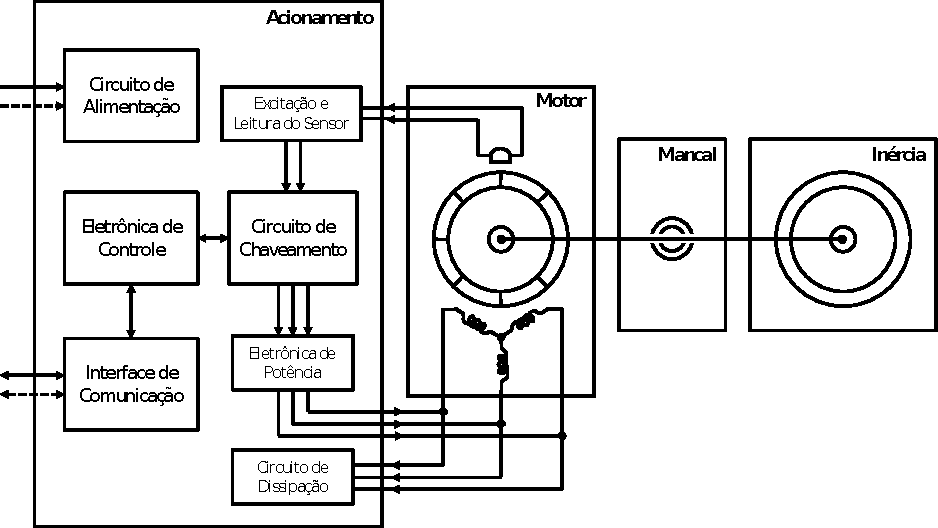
\includegraphics[width=1\linewidth]{./Figs/EsquemaRoda}
\caption{Esquema geral de uma roda de reação}
\label{fig:EsquemaRoda}
\end{figure}

O controle de atitude  com rodas de reação demanda que esse tipo de  atuador opere em toda sua escala de velocidade, inclusive na inversão de seu sentido de rotação (passagem pelo zero), de uma forma estável e controlada. A zona morta, efeito do atrito estático do mancal, deve ser minimizada a fim de se obter um bom funcionamento da roda de reação. A zona morta pode ser compensada (no caso do mancal por rolamento) pela implementação de leis de controle com malhas de velocidade e corrente, além de um estimador de atrito \citep{Carrara2010}.

O projeto de uma roda de reação começa pelo estudo e definição do momento angular a ser utilizado na roda de reação, essa escolha leva em consideração os distúrbios sofridos pelo satélite e a precisão necessária na missão. Com o momento angular definido, especifica-se a inércia e então o mancal, por último projeta-se um motor capaz de girar o conjunto mancal mais inércia.

\section{Objetivo}

Essa dissertação acompanha o esforço de projetar um mancal magnético para uma roda de reação que está sendo desenvolvida no Núcleo de Sistemas Eletrônicos Embarcados (NSEE) do Instituto Mauá De Tecnologia (IMT) com apoio do Instituto Nacional De Pesquisas Espaciais (INPE).

O projeto, envolve o desenvolvimento de uma topologia capaz de ser utilizada numa roda de reação para satélites de médio porte, mais especificamente, para a plataforma multi missão.


\section{Justificativa}

A suspensão do rotor com relação ao estator representa uma parte crítica em rodas de reação \citep{taniwaki2003experimental} devido às consequências de qualquer fricção no movimento relativo entre estes dois componentes. Com efeito, a fricção se traduz não apenas em um maior consumo de potência elétrica como também na introdução de uma zona morta de atuação em torque, bem como na limitação da vida útil da roda de reação devido ao gradual desgaste do mancal.

Uma solução mecânica para a interface entre o rotor e o estator é o mancal por rolamento. Apesar de sua aparente simplicidade, apresenta desafios para a obtenção dos valores mínimos de fricção necessários, em vista das exigências de consumo, controlabilidade e vida útil da roda de reação \citep{Krishnan2010}. No caso de aplicações aerospaciais, a lubrificação do rolamento representa também considerável dificuldade devido à impossibilidade de utilização de lubrificantes tradicionais em condições de baixa ou nenhuma pressão atmosférica, que leva à perda dos componentes voláteis destes lubrificantes e sua consequente degradação. Outra dificuldade se deve à tendência de migração dos lubrificantes na ausência de gravidade, o que costuma ser abordado com estratégias de recaptura ou relubrificação. Sistemas desse tipo, apresentam grande complexidade e seu comportamento orbital é de difícil validação em laboratório.

As dificuldades associadas ao uso de mancal de rolamento residem também em sua modelagem, consequência da variação de viscosidade do lubrificante em função da temperatura do mancal, o que torna o coeficiente de fricção dependente da velocidade de rotação e das condições térmicas em geral \citep{Carrara2007}. O mancal por rolamento apresenta, por outro lado, grande vantagem construtiva devido à compactação do sistema e não necessidade de eletrônica extra para o seu controle. 

Para contornar os problemas de lubrificação em baixa pressão, algumas rodas de reação  utilizam um sistema hermeticamente selado pressurizado com um gás inerte \citep{Krishnan2010}. Esta solução relaxa os requisitos de lubrificação, porém impõe uma força de arrasto extra na roda e não resolve o problema da migração dos lubrificantes na ausência de gravidade. Uma pesquisa detalhada dos lubrificantes de classe espacial e estratégias de selamento e relubrificação deve ser realizada.

Outra solução é a utilização de um mancal magnético \citep{Bangcheng2012}, que é uma alternativa sem contato mecânico entre o rotor e o estator, pela qual o rotor é mantido suspenso magneticamente. O ganho em confiabilidade e vida útil da roda de reação é considerável \citep{Marble2006}, sendo a vida útil basicamente limitada  pela durabilidade da eletrônica. A operação sem contato elimina a necessidade de lubrificante e possibilita consequentemente a operação em vácuo, o que se traduz em simplificação nos requisitos da concepção mecânica. 

A ausência de fricção faz com que deixe de existir a zona morta de aplicação de torque em baixas velocidades, eliminando não-linearidades da lei de controle, além de possibilitar a diminuição da causa de defeitos de balanceamento e vibrações mecânicas. Consequentemente, gera um ganho em simplicidade dos algoritmos e em desempenho do controle de atitude. A contrapartida é a adição de uma malha ou mais de controle para a suspensão eletromagnética. O ganho de eficiência trazido pela ausência de fricção também é contrabalançado, ao menos parcialmente, pelo consumo de potência dos atuadores deste tipo de mancal.


\section{Revisão bibliográfica}


Estudo iniciais sobre mancais magnéticos são datados do século XIX \citep{Weise1989}, porém só recentemente começaram a ter grandes aplicações na sociedade. Essas aplicações vão desde motores de alta eficiência até equipamentos médicos. Mancais magnéticos fazem uso extensivo de campos magnéticos e tiveram uma grande evolução quando os ímãs de terras raras tornaram-se acessíveis, possibilitando o aumento da geração de campos magnéticos permanentes \citep{Furlani2001}.

Mancais magnéticos podem ser classificados em dois grandes grupos: os que utilizam da \textit{força de relutância} e os que utilizam da \textit{força de Lorentz}. O primeiro grupo é chamado de mancais magnéticos ativos (em inglês, AMBs) e o segundo são os mancais magnéticos passivos (PMBs) \citep{Schweitzer2009}.

Os AMBs funcionam com um controle ativo de algumas das forças atuantes no mancal a fim de estabilizar o sistema (controle em malha fechada). Já os mancais puramente passivos geram as forças necessárias para estabilizar o rotor apenas via ímãs.
Mancais magnéticos puramente passivos (seis graus de liberdade) que utilizam somente ímãs são impossíveis, dado que sempre um dos graus de liberdade torna-se instável (Teorema de Earnshaw's) \citep[pg. 20]{Schweitzer2009}.


\subsection{Graus de liberdade}

Os mancais magnéticos podem ser classificados pelo número de graus de liberdade controlados ativamente \citep{Schweitzer2009}:

\begin{enumerate}[a)]
	\item  Mancal puramente passivo
	
	Este mancal totalmente passivo é formado por um rotor contendo um conjunto de imãs permanentes em disposição de Halbach \citep{Detoni2012}, o que gera potencialização do campo magnético adjacente ao rotor. Um conjunto de enrolamentos passivos no estator é excitado por esse campo magnético girante. Na eventualidade de qualquer deslocamento do rotor, o enrolamento reage com o campo magnético, gerado pela atração/repulsão do rotor, ocasionando a volta à posição de equilíbrio. O sistema é estável a partir de uma velocidade de rotação mínima do rotor (velocidade crítica). O fato desta topologia não funcionar em baixas velocidades angulares a torna pouco adaptada para aplicação em rodas de reação.
	
	\item  Mancal ativo num grau de liberdade
	
	Nesse caso, o rotor é levitado em apenas um de seus grau de liberdade, necessitando que os demais graus de liberdade sejam estabilizados externamente (com por exemplo o uso de mancais mecânicos). Trata-se de uma configuração que necessita de uma eletrônica de controle relativamente simples e de baixo consumo de potência.
	
	\item Mancal ativo em dois graus de liberdade
	
	Aqui, o rotor e o estator compõem um circuito magnético em configuração atrativa, em geral com ímãs permanentes no rotor acoplados a um circuito magnético de baixa relutância no estator. O sistema é estável axialmente mas necessita controle ativo na direção radial. Essa configuração resulta num mancal de boa rigidez radial, com arquitetura simplificada e pequenas dimensões, principalmente na direção longitudinal.
	
	\item Mancal ativo em cinco graus de liberdade
	
	Este mancal totalmente ativo é formado por atuadores eletromagnéticos nas duas direções radiais, na direção axial e nos dois modos de rotação radiais. A principal vantagem de sua aplicação em rodas de reação é a possibilidade de atuação em mais de um eixo de rotação, devido à capacidade de manobra do componente de inércia. Trata-se no entanto de um sistema de controle de grande complexidade, com consequente redução de confiabilidade. 
\end{enumerate}

\subsection{Topologias com Aplicação em Rodas de Reação}

Encontram-se na literatura três topologias distintas para utilização de mancais magnéticos em rodas de reação. Os mancais propostos para esse tipo de aplicação possuem, em sua maioria, dois graus de liberdade ativos e fazem uso de ímãs permanentes para a geração de campos magnéticos para minimizar o consumo elétrico ativo do sistema. Em seguida, analisamos os principais pontos desses mancais.

A topologia proposta por \citet{Bernus1998} trabalha com dois graus de liberdades ativos, com ímãs permanentes no rotor e dois estatores: um interno com bobinas para o controle do fluxo magnético no rotor (por consequência na direção radial) e outro externo para estabilização axial que também contribui com a rigidez axial. 

Nessa topologia (Fig. \ref{Fig:modelo:frances}), um fluxo magnético contínuo é gerado no rotor por ímãs permanentes ali instalados, as bobinas no estator interno conseguem gerar campos aditivos e subtrativos no rotor (dependente do sentido da corrente). Se o campo for aditivo, pode-se aumentar a rigidez do eixo longitudinal, caso o campo for subtrativo, consegue-se diminuir sua rigidez, tornando assim mais fácil o deslocamento radial do rotor.

\begin{figure}[!ht]
	\centering
	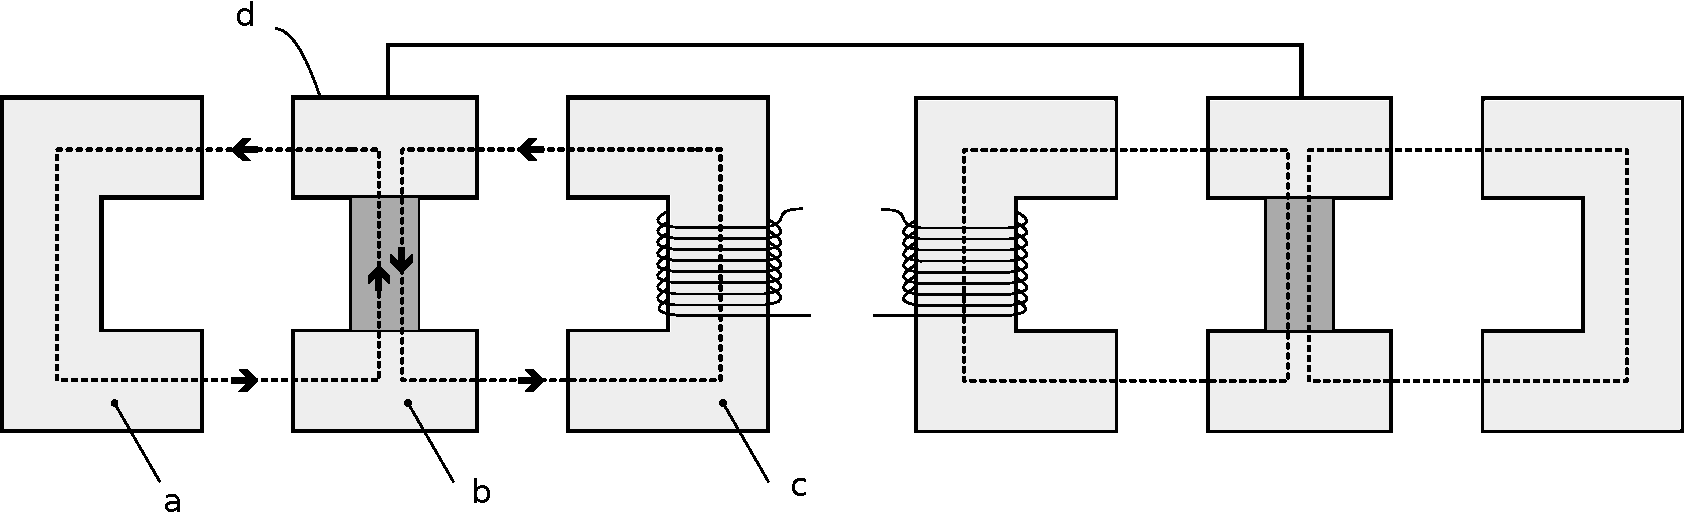
\includegraphics[width=1\linewidth]{./Figs/mancais/frances}
	\caption{Corte da topologia proposta por \cite{Bernus1998} \\
	a: estator externo; b: rotor; c: estator interno; d: ímãs permanentes}
	\label{Fig:modelo:frances}
\end{figure}

A topologia proposta por \citet{Scharfe2001} difere por ter somente um estator e pelos ímãs permanentes estarem localizados no estator e não no rotor. Como ilustrado na Fig. \ref{Fig:modelo:alemao}. 

%\todo[inline]{falar mais ...}

\begin{figure}[!ht]
	\centering
	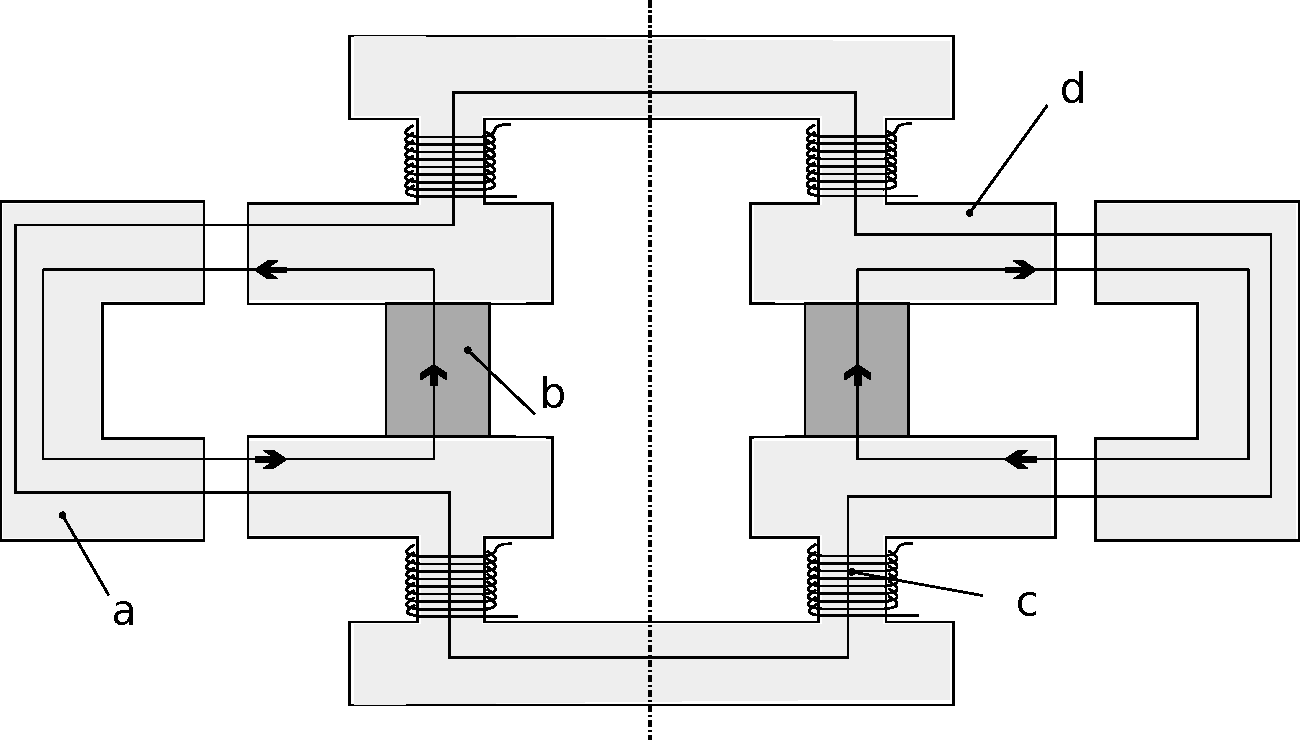
\includegraphics[width=0.8\linewidth]{./Figs/mancais/alemao.pdf}
	\caption{Corte da topologia proposta por \cite{Scharfe2001} \\
	a: estator externo; b: rotor; c: estator interno; d: ímãs permanentes}
	\label{Fig:modelo:alemao}
\end{figure} 

Com essa arquitetura é possível utilizar as bobinas tanto para exercer uma força atrativa no rotor quanto para tornar a sua rigidez mais branda, facilitando a atração do rotor. É possível também aumentar a rigidez axial por permitir a inserção um fluxo positivo em ambas as bobinas, esse fluxo soma-se com o fluxo gerado pelos ímãs permanentes.

Mais recentemente, uma nova arquitetura foi proposta por \citet{Bangcheng2012} para ser utilizada em uma roda de reação de um satélite ágil.  O rotor é composto de duas partes, uma externa utilizada para estabilizar o mancal na direção axial e outra interna para controle de posição na direção radial. Diferente das outras propostas, essa não utiliza um perfil em "C" para estabilização dos graus de liberdade passivos, mas sim, faz uso de um perfil plano com ímãs permanentes tanto no rotor quanto no estator.  Ímãs permanentes também são usados nos polos do mancal, esses criam um fluxo (\textit{bias}) constante diminuindo a corrente necessária para controlar o rotor.
 
%\begin{figure}[!ht]
%	\centering
%	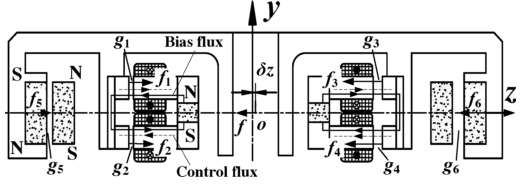
\includegraphics[width=1\linewidth]{./Figs/mancais/chines}
%	\caption{Corte da topologia proposta por \cite{Bangcheng2012}}
%	\label{Fig:modelo:chines}
%\end{figure}

\subsection{Modelagem Eletromagnética}

Devido às não linearidades do mancal magnético (por exemplo a sua rigidez em função do deslocamento), a modelagem analítica é de difícil obtenção e uma abordagem por elementos finitos é recomendada \citep{pilat2007automatic}. Com esse tipo de análise é possível verificar o acoplamento das forças e momentos envolvidos além das características térmicas do sistema.

Modelos analíticos \citep{Tezuka2013, Chiba} auxiliam no entendimento e na escolha dos parâmetros construtivos e magnéticos do mancal. A solução de um modelo analítico quando comparada à de um modelo com elementos finitos é computacionalmente mais rápida.

Com o modelo analítico é possível a utilização de métodos de otimização \citep{Wu2009, Fang2014} para a obtenção de um mancal com melhores propriedades, dentre elas, menor potência, maior rigidez e dimensões dentro das especificações. 

\subsection{Sensoriamento}

Devido ao controle da posição do rotor em mancais magnéticos, o sensoriamento de sua posição é essencial para o funcionamento do sistema. Duas linhas de sensoriamento são encontradas na literatura: mancais auto sensoriados \citep{Vischer1993} e os que utilizam sensores de posição dedicados para esse fim.

Os mancais magnéticos sem sensores (\textit{sensorless}) utilizam geralmente as bobinas de seus polos para sensoriar a posição do rotor. Diversas técnicas podem ser empregadas \citep{Hofer2009a, Mukhopadhyay2005} entre elas: medição da indutância dos polos pela injeção de um sinal com uma portadora de frequência mais elevada ou a medição da força contra-eletromotriz induzida nas bobinas.
 
Já os mancais sensoriados utilizam sensores de deslocamentos exclusivos para a medição da posição do rotor e, por consequência, do tamanho do entreferro \citep{Sivadasan1996}. Os sensores podem ser de dois tipos: capacitivos ou indutivos, dependendo do material construtivo do sistema. Opera-se geralmente com sensores na distribuição diferencial, visando minimizar os efeitos de suas não linearidades.
 
\subsection{Mancais auxiliares}

 Mancais auxiliares são importantes em mancais magnéticos, pois são eles que evitam colisões entre as partes fixas e as rotativas em caso de algum tipo de falha. Mancais magnéticos projetados para operar em altas rotações não possuem bom rendimento na inicialização  (baixa rotação) e se utilizam dos mancais auxiliares nessa zona até atingirem a sua velocidade de operação. Os mancais auxiliares podem ser compostos por rolamentos esféricos \citep{Sun2004a} ou por elementos sólidos auto-lubrificantes como Teflon.
 
\subsection{Técnicas de controle}

O controle de mancais magnéticos é uma área fértil da engenharia de controle, as não linearidades do sistema tornam os projetos nada triviais.  

Técnicas de controle clássicas são utilizadas com bastante frequência em mancais magnéticos. Controle do tipo PID \citep{Tezuka2013} possui ampla utilização pela sua fácil implementação na forma analógica e consolidada técnica. O controle  do tipo \textit{feedforward} é utilizado em casos onde há o acoplamento entre os graus de liberdade, podendo ser utilizado para o desacoplamento dos mesmos. Outras técnicas propostas na literatura situam-se na área de controle multivariável, e fazem uso de controle robusto \citep{Jimenez-Lizafrraga2007}, controle ótimo \citep{Schuhmann2012} e controle não linear \citep{Rundell1996}.

\subsection{Eletrônica}

A eletrônica em sistemas espaciais consiste normalmente de uma parte crucial do sistema, sendo bastante sensível aos efeitos da radiação \citep{Stassinopoulos1988}. Falhas em sensores, por exemplo, representam um dos maiores problemas para o bom funcionamento de sistemas aeroespaciais em seu pleno potencial \citep{Balaban2009}, e estão muitas vezes relacionadas ao cancelamento de missões devido ao mau funcionamento de sistemas. Além dos sensores, memórias podem ter seus dados alterados devido ao impacto de uma partícula de alta energia, podendo causar falha crítica no sistema.

\section{Metodologia}

A metodologia adotada neste trabalho envolve a utilização de simulações em elementos finitos para o desenvolvimento das partes magnéticas do mancal, uma modelagem fenomenológica foi feita para a realização da otimização dos parâmetros físicos do sistema. 

O desenvolvimento do projeto foi executado como ilustrado na Fig. \ref{fig:metodologia:fluxo:dev}, onde primeiramente as especificações de projeto foram levantadas e uma topologia de mancal proposta com base no levantamento bibliográfico. 

Um protótipo foi construído a fim de avaliar a topologia proposta, verificou-se com ele que as premissas de estabilidade e força foram alcançadas. A construção desse protótipo foi realizada na oficina mecânica da Escola de Engenharia Mauá (EEM). Devido a ausência de fomento, a prototipagem não pode ser efetuada seguindo todas as especificações de rigor mecânico, o que gerou falhas na montagem.

O material utilizado também foi influenciado por esse fator, utilizou-se no caso o aço 1020 para as partes magnéticas (de amplo uso comercial) e alumínio para as partes não magnéticas. 

Na etapa de otimização, dividiu-se o projeto em duas partes: na primeira considerou-se somente a parte passiva (estator externo e rotor) até que um conjunto com rigidez suficiente na direção axial e com menor força de atração na direção radial fosse atingido. Com esses valores buscou-se um estator interno capaz de exercer força de atração suficiente no rotor para estabilizá-lo em seu ponto de operação.

Com um modelo em elementos finitos (FEM) calculou-se com exatidão os parâmetros magnéticos do mancal proposto a serem utilizados na modelagem dinâmica do rotor.

Com o modelo dinâmico, um controlador capaz de estabilizar o rotor em seu ponto de operação foi proposto, com ele, mostrou-se a viabilidade de controlar o mancal dentro das restrições de potência propostas. 

A Fig. \ref{fig:metodologia:fluxo:dev} mostra o fluxo do desenvolvimento do mancal.

 
\begin{figure}[th!]
	\centering
	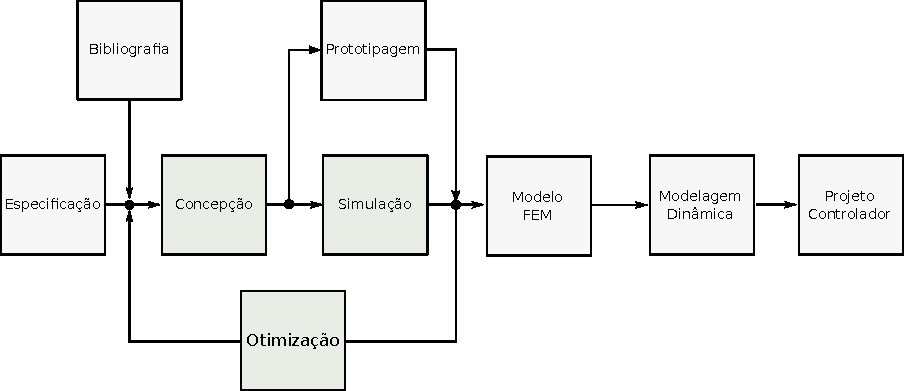
\includegraphics[width=1\linewidth]{Figs/metodologia_fluxo_dev}
	\caption{Fluxo de desenvolvimento}
	\label{fig:metodologia:fluxo:dev}
\end{figure} 
 
\section{Sumário Estruturado}
 
No segundo capítulo, o mancal magnético proposto foi descrito e suas propriedades construtivas apresentadas. Nele podemos verificar conceitualmente todos os componentes que constituem o sistema proposto.

O capítulo 3 apresenta um modelo não linear para representar a interação entre o estator externo e o rotor. Esse conjunto é responsável pela estabilização do rotor nos graus de liberdades passivamente estáveis. No modelo analítico foi aplicada uma otimização nos parâmetros construtivos do mancal visando encontrar um mancal compacto e com boa rigidez passiva. A partir de um modelo em elementos finitos obteve-se as relações de força por deslocamento.

No capítulo 4 desta dissertação, um modelo fenomenológico que modela a interação entre o estator interno e o rotor está apresentado. Similarmente ao capítulo anterior, foi aplicada uma otimização visando a obtenção dos parâmetros construtivos do estator interno. Com o modelo em elementos finitos, chega-se às equações de força resultante dessa otimização do mancal.  

No quinto capítulo, a partir das dimensões e das equações de forças definidas anteriormente, um modelo dinâmico para o rotor está apresentado. Esse modelo foi utilizado para o projeto de uma malha de controle capaz de estabilizar o rotor em seu ponto de operação.

O último capítulo constitui-se de uma revisão do desenvolvimento da dissertação e apresentação de considerações finais sobre o projeto.


